%%!TEX TS-program = pdflatexmk
%%!TEX encoding = UTF-8 Unicode
\documentclass[11pt,french]{article}
\usepackage[utf8]{inputenc}
%\usepackage[body={6.0in,9.0in}, vmarginratio=1:1]{geometry}
\usepackage[a4paper,twoside,textheight=25.1cm,heightrounded]{geometry} % allonge le texte, hors proportions
\usepackage[small,compact]{titlesec}

%%\usepackage[expert]{fourier}
%\usepackage{fourier}
%\usepackage[scaled=0.85]{berasans}
%\usepackage[scaled=0.85]{beramono}

\usepackage{booktabs}

% Include graphicx
\usepackage{graphicx}
%\usepackage{applekeys}

%\usepackage{microtype}
\usepackage{varioref}

\usepackage{xcolor}
%\usepackage[colorlinks, urlcolor=darkgray, linkcolor=darkgray]{hyperref}


%\newcommand{\MacTeX}{Mac\TeX}
\newcommand{\MacTeX}{Mac\kern-.12em\TeX}
\newcommand{\BibTeX}{B\textsc{i\kern-.025em  b}\kern-.13em\TeX}
\newcommand{\conTeXt}{Con\kern-.12em\TeX t}
\newcommand{\TS}{\textsf{\TeX Shop}}
% default small caps used for utopia are ugly; don't want to use [expert] here.
%\newcommand{\acr}[1]{\textsc{#1}}
%\usepackage{relsize}
%\newcommand{\acr}[1]{\textrm{\smaller\uppercase{#1}}}
\newcommand{\acr}[1]{\textsf{#1}}
%\newcommand{\cmd}[1]{\texttt{#1}}
%\newcommand{\mnu}[1]{\texttt{#1}}
\newcommand{\cmd}[1]{\textsf{#1}}
\newcommand{\mnu}[1]{\textsf{#1}}
\newcommand{\To}{\,\(\to\)\,}

% set | as a command character within verbatim so you can execute commands there
\usepackage{verbatim}
\makeatletter
\addto@hook\every@verbatim{\catcode`|=0}
\makeatother

% define colored items to be inserted in verbatim environments
\setlength{\fboxsep}{0pt}
\newcommand{\selmark}{\colorbox{green}{\rule[-0.5ex]{0ex}{2.1ex}\texttt{•}}}

%\usepackage[expert]{fourier}
\usepackage{fourier}
\usepackage[scaled=0.85]{berasans}
\usepackage[scaled=0.85]{beramono}

%Babel
\usepackage{babel}
\addto\captionsfrench{\def\tablename{\scshape Tableau}}
\frenchbsetup{ShowOptions,og=«,fg=»}
\usepackage{xfrac}
\usepackage[decimalsymbol=comma,unitsep=cdot,digitsep=thick,mode=text,sepfour=true,valuesep=thick]{siunitx}
\usepackage[np,autolanguage]{numprint}

%Caption, float, microtype
\usepackage{caption,float}
\usepackage[final,babel]{microtype}

%HYPERREF
\usepackage[colorlinks=true,linkcolor=black,urlcolor=blue]{hyperref}


\title{Conseils et astuces pour \TS\\\small v0.5.0--2011/04/20\thanks{Traduit par René Fritz le 26 avril 2011.}}
\author{H. Schulz\\\small\href{mailto:herbs2@mac.com}{herbs2@mac.com}}
\date{}

\begin{document}
\maketitle

\tableofcontents

\newpage

\section{Introduction}

\TS\ est une « interface » \emph{(Front End)} pour une distribution \TeX\ sur Mac OS~X. Il permet de créer et d'éditer des fichiers source \TeX{}, d'interagir avec la distribution \TeX\ (p. ex., composer le fichier source) et enfin de donner un aperçu du fichier \acr{pdf} final. Il permet également d'aller et venir entre l'aperçu et le source.

%\TS\ is a ``Front End'' for a \TeX\ distribution on Mac OS~X. As such it allows the user to create and edit \TeX\ source files, interact with the \TeX\ distribution (e.g., typeset the source file) and, finally preview the final \acr{pdf} file. It also allows the user to go back and forth between preview and source.

Au fil des ans \TS\ a ajouté de nombreuses fonctionnalités. Certaines d'entre elles sont claires et sont destinées à aider un novice à ses débuts. D'autres sont un peu plus subtiles dans leur utilisation et leur puissance sous-jacente doit être apprivoisée.

%Over the years \TS\ has added many features. Some of them are obvious and are meant to help a novice get started. Others are a bit more subtle in their use and the underlying power of these features needs to be coaxed out.

\subsection{Ce que vous ne trouverez pas ici}
%\subsection{What Isn't Here}

Tout d'abord, cet article \emph{ne traite pas} de \TeX\ ou \LaTeX. Je n'ai pas l'intention de vous apprendre à écrire un source \TeX{}. Il y a beaucoup de livres et articles bien faits qui vous enseigneront comment devenir un \TeX pert\footnote{Un expert en \TeX.} ou, du moins, un \TeX pätzer\footnote{\emph{Pätzer}, désigne un mauvais joueur d'échecs.} comme moi.
 
Bien qu'il renferme des éléments d'introduction, il n'est cependant \emph{pas} conçu comme un manuel exhaustif sur \TS\ pour les nuls. Au fil du temps, il pourrait évoluer vers un tel document, mais je dois commencer quelque part et je n'en suis qu'au début.

%This article is, first of all, \emph{not} about \TeX\ or \LaTeX. I don't intend to teach you how to write \TeX\ source. There are many fine books and articles that will teach you how to become a \TeX pert or, at least, a \TeX pätzer like me.
%
%Although there is some introductory material it is also \emph{not} meant as a complete manual for the use of \TS\ for the total novice. Over time it might evolve into such a document but I've got to start somewhere and this is that start.

\subsection{Ce qui est ici}
%\subsection{What Is Here}

Dans cet article, je souhaite vous présenter quelques-unes des subtilités qui rendront votre vie d'éditeur de source \TeX\ plus facile. Il s'agit, notamment, d'ajouter des commandes de clavier et d'étendre les capacités d'édition de \TS{} ; d'alléger votre travail dans la création de documents, etc., en utilisant des macros et le complètement de commande ; et, enfin, de savoir comment on peut étendre les capacités de traitement de \TS\ grâce aux moteurs.

%In this article I hope to introduce you to some of the more subtle things you can do to make your life as a \TeX\ source editor easier. These include adding keyboard commands and extending the editing capabilities of \TS; helping you make short(er) work of creating documents, etc., with the use of Macros and Command Completion; and, finally, how one can extend the processing capabilities of \TS\ using Engines.

\section{Édition, composition et visualisation --- le cycle de travail}
%\section{Editing, Typesetting and Viewing --- the Work Cycle}

Dans ce document, c'est la section la plus proche des débutants.

%This is about as close to a beginner's section you will get in this document.

\subsection{Édition du fichier source}
%\subsection{Editing the Source File}

La première chose que vous ayez à faire pour créer ce grand ouvrage est de le taper dans le document source qui sera composé et visualisé plus tard. Ceci nécessite d'entrer, à la fois, le balisage \LaTeX\ ainsi que vos merveilleux mots dans le document.

%The first thing you've got to do to create that great work is to type it into the source document that will be typeset and viewed later. This involves both putting \LaTeX\ markup as well as your wonderful words into the document.

Pour démarrer, vous pouvez ouvrir un nouveau document en utilisant \mnu{Fichier}\To\mnu{Nouveau} (\cmd{Cmd-N}), puis en remplir le début en choisissant un modèle dans le menu déroulant \mnu{Modèles} situé dans la fenêtre du source ou utiliser --- nouveau avec \TS\ 2.36 --- la commande \mnu{fichier}\To\mnu{Nouveau depuis la papeterie…} et choisir le source adéquat dans la liste. Notez que la liste des modèles et des articles fournis dans la papeterie est incomplète, si vous en avez dont vous pensez qu'ils seraient très utiles, n'hésitez pas à les soumettre pour inclusion dans \TS. Vous pouvez ajouter vos modèles et sources personnels dans \path{~/Library/TeXShop/Templates/} et dans \path{~/Library/TeXShop/Stationery/}. \textbf {Note : \path{~/Library/} est le dossier \texttt{Library} dans votre dossier \texttt{HOME}.}

%To get started you can open a new document using \mnu{File}\To\mnu{New} (\cmd{Cmd-N}) and then fill in the start of a new document by choosing a template from the \mnu{Templates} popup menu in the Source Window or use---new with \TS\ 2.36---the \mnu{File}\To\mnu{New From Stationery…} command and picking appropriate Stationery from the list. Note that the templates and stationery provided are certainly not complete; if you have some that you think are of general use feel free to submit them for inclusion in \TS. You can add personal Templates and Stationery to \path{~/Library/TeXShop/Templates/} and \path{~/Library/TeXShop/Stationery/} respectively. \textbf{Note: \path{~/Library/} is the \texttt{Library} folder in your \texttt{HOME} folder.}

\subsubsection{Palettes LaTeX et Matrice}
%\subsubsection{\LaTeX\ \& Matrix Panels}

Même si je crois que les panneaux avec une interface cliquable font réellement obstacle à l'apprentissage, je vais mentionner que \TS\ a deux panneaux d'aide à la saisie du code \LaTeX\ (la \mnu{Palette LaTeX…}) et à la mise en place de la structure de base d'une matrice ou d'un tableau (la \mnu{Palette Matrice…}). Ils sont activés ou désactivés dans le menu \mnu{Fenêtre} ou avec les raccourcis clavier\footnote{Les raccourcis sont donnés pour un clavier anglais et peuvent être différents pour d'autres claviers.} \texttt{Opt-Cmd-{}-} et \texttt{Opt-Cmd-=} respectivement. La \textsc{Figure}~\ref{fig:LandMPanels} montre l'aspect de ces panneaux.
%While I believe that panels with a clickable interface actually hinder learning I'll mention that TeXShop has two panels to help with entering \LaTeX\ code (the \LaTeX\ Panel) and for setting up the basic structure of a matrix or tabular (the Matrix Panel). These are toggled on/off under the \mnu{Window} Menu or with the keyboard shortcuts\footnote{The given shortcuts are for the English localization and may be different with other localizations.} \texttt{Opt-Cmd-{}-} and \texttt{Opt-Cmd-=} respectively. Figure (\ref{fig:LandMPanels}) shows what the panels look like.
\begin{figure}
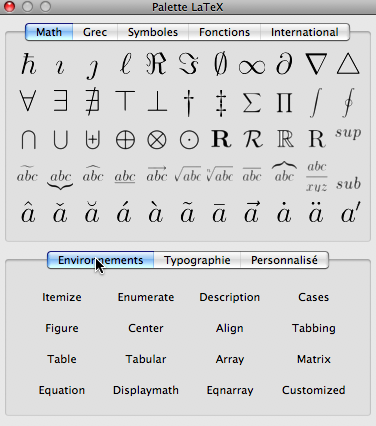
\includegraphics[width=2.5in]{figs/palette}\hfill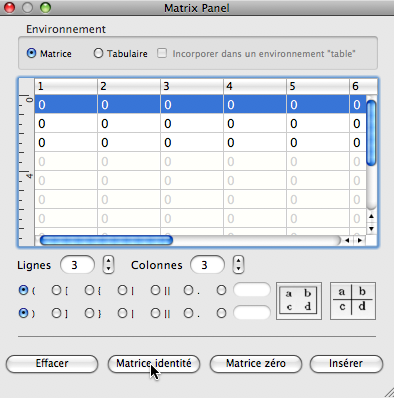
\includegraphics[width=2.5in]
{figs/matrice}
\caption{Les panneaux LaTeX et Matrix.\label{fig:LandMPanels}}
\end{figure}
Il est possible de faire quelques modifications et ajouts à la palette LaTeX  en modifiant le fichier \path{~/Library/TeXShop/LatexPanel/completion.plist}. \textbf{Note : tous les fichiers \path{plist} doivent être édités en utilisant le codage Unicode UTF-8.}

%It is possible to make a few changes and additions to the \LaTeX\ Panel by editing the 
%\path{~/Library/TeXShop/LatexPanel/completion.plist} file. \textbf{Note: all \path{plist} files must be edited using UTF-8 Unicode encoding.}

\subsubsection{Liste du menu Étiquettes}
%\subsubsection{The Tags Popup}

Le menu déroulant \mnu{Étiquettes} de la barre d'outils du source liste automatiquement les commandes de sectionnement pour vous permettre de passer rapidement à une partie pertinente du source de votre document. Vous pouvez ajouter votre propre étiquette à un endroit particulier de cette liste en plaçant dans le document la ligne
%The \mnu{Tags} popup menu on the Source Toolbar will automatically list sectioning commands so you can quickly jump to a relevant part of your document source. You can add your own tag to the list at a particular place in the document by placing the line
\begin{verbatim}
%:le nom de mon étiquette
\end{verbatim}
et elle apparaîtra alors à cette position dans la liste déroulante et, ainsi, vous pourrez sauter rapidement à cet endroit. Voir la \textsc{Figure}~\ref{fig:Tags}. Désolé, les balises ne sont pas incluses de manière récursive pour les fichiers que vous incluez par \verb|\include| ou \verb|\input|.

%at that position and it will then appear in the popup list so you can jump to that location quickly. See Figure (\ref{fig:Tags}). Sorry, tags are not recursively included for files you \verb|\include| or \verb|\input|.
\begin{figure}
\centering
\framebox{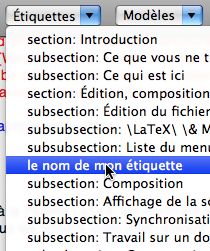
\includegraphics[width=1.5in]{figs/etiquette}}
\caption{Liste du menu Étiquettes.\label{fig:Tags}}
\end{figure}

\subsection{Composition}
%\subsection{Typesetting}

Une fois que vous êtes prêt à jeter un \oe{}il sur la façon dont votre document apparaîtra vous composerez avec le moteur défini par défaut, \texttt{pdflatex}, en allant simplement dans le menu \mnu{Composition}\To\mnu{Composer} (\cmd{Cmd-T}).

Vous pouvez utiliser un moteur différent de celui défini par défaut. Pour faire ce changement allez dans \mnu{TeXShop}\To\mnu{Préférences…}\To\mnu{Composition}.

Si vous incluez beaucoup de fichiers graphiques \acr{eps} dans votre document vous pouvez réaliser la composition en utilisant \texttt{latex}\To\texttt{dvips}\To\texttt{ps2pdf} car \texttt{pdf(la)tex} ne permet pas d'inclure directement les fichiers \acr{eps}\footnote{Le programme \texttt{pdflatex} à partir de \MacTeX-2010 peut faire, au vol, cette conversion des fichiers \acr{eps}.}. La meilleure façon de le faire est d'entrer la ligne
\begin{verbatim}
%%! TEX TS-program = latex
\end{verbatim}
en tête de votre document. Alors, \TS\ composera avec la méthode \texttt{latex+distiller}, notée ci-dessus, quel que soit le réglage du moteur par défaut. Remplacez \texttt{latex} par \texttt{pdflatex} pour forcer l'utilisation de \texttt{pdflatex} pour composer votre fichier.

%Once you are ready to take a look at how your document will appear you typeset it with the default engine, \texttt{pdflatex} out of the box, by simply using the \mnu{Typeset}\To\mnu{Typeset} (\cmd{Cmd-T}) command.
%
%You may wish to use a different engine as your default. You can change the default engine in \mnu{TeXShop}\To\mnu{Preferences}\To\mnu{Typesetting}.
%
%If you are including many \acr{eps} graphics files in your document you may wish to typeset using \texttt{latex}\To\texttt{dvips}\To\texttt{ps2pdf} since \texttt{pdf(la)tex} does not allow for direct inclusion of \acr{eps} files\footnote{The \texttt{pdflatex} program in \MacTeX-2010 and later will do on-the-fly conversion of \acr{eps} files.}. The easiest way to do this is to include the line
%\begin{verbatim}
%% !TEX TS-program = latex
%\end{verbatim}
%at the top of your document. Then \TS\ will use the \texttt{latex+distiller} typesetting method noted above no matter what the default engine setting. Change \texttt{latex} to \texttt{pdflatex} to force use of \texttt{pdflatex} to typeset your file.

\subsection{Affichage du fichier \acr{pdf}}
%\subsection{Viewing the Output \acr{pdf} File}

En supposant que le document a été composé correctement, le fichier \acr{pdf} s'ouvre automatiquement dans une fenêtre d'aperçu distincte.

Vous pouvez contrôler la façon dont il est affiché dans le menu \mnu{Page} et modifier les paramètres par défaut dans \mnu{TeXShop}\To\mnu{Préférences…}\To\mnu{Aperçu du PDF}.

%Assuming the document was successfully typeset the \acr{pdf} file will automatically open in a separate preview window.
%
%You can control how it's displayed in the \mnu{Preview} Menu. You can change the default settings in \mnu{TeXShop}\To\mnu{Preferences}\To\mnu{Preview}.

\subsubsection{Synchronisation entre le \acr{pdf} et le source}
%\subsubsection{Synchronizing between \acr{pdf} and Source}

Avec les distributions \TeX\ les plus récentes, vous pouvez également aller d'un emplacement dans la fenêtre de l'aperçu à l'emplacement correspondant dans la fenêtre du source, et inversement, par la commande clavier \cmd{Cmd-clic}. Voir la \textsc{Figure}~\ref{fig:SourcePreviewSync} pour un exemple de synchronisation source\To aperçu et aperçu\To source.


%With more recent \TeX\ distributions you can also skip back and forth between a location in the Preview Window and the equivalent location in the Source Window by \cmd{Cmd-Clicking} in either one to go to the (approximate) location in the other. See Figure (\ref{fig:SourcePreviewSync}) for an example of Source\To Preview and Preview\To Source synchronization.

\begin{figure}
\centering
\framebox{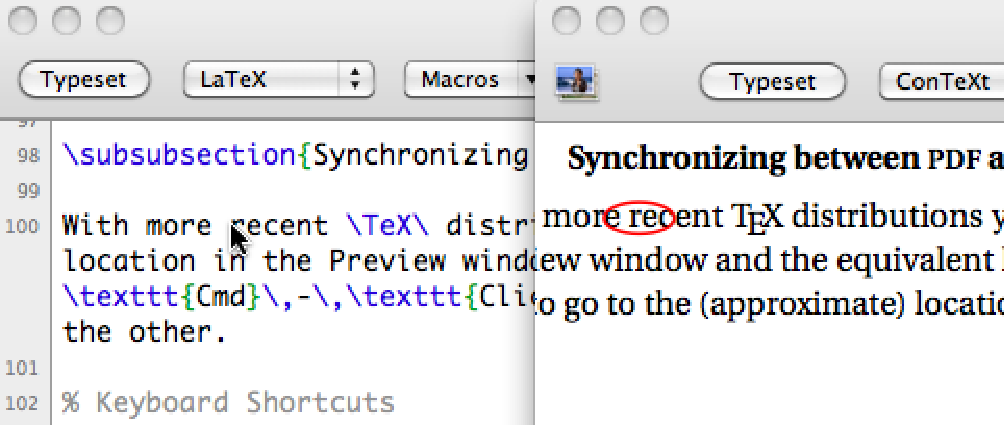
\includegraphics[width=.475\textwidth]{figs/SourceToPreviewSync}}\qquad\framebox{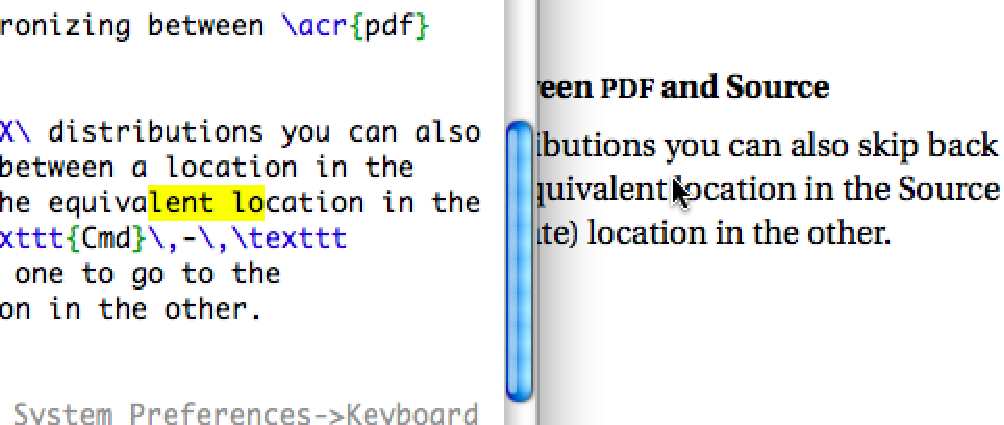
\includegraphics[width=.475\textwidth]{figs/PreviewToSourceSync}}
\caption{Synchronisation source\To aperçu et aperçu\To source.\label{fig:SourcePreviewSync}}
\end{figure}

\subsection{Travail sur un document volumineux}
%\subsection{Working with a Large Document}

Il est souvent utile de diviser un document de grande taille en plusieurs parties subalternes plus faciles à gérer, puis de créer un fichier « principal » qui contient le préambule et des commandes \verb|\include| pour réunir toutes les parties lors de la composition.

Pour que \TS\ « sache » quel fichier il doit composer lorsque vous travaillez sur un fichier secondaire entrez la ligne \begin{verbatim}
% !TEX root = path/to/rootfile.tex
\end{verbatim}
en tête de votre fichier secondaire ; \path{path/to/rootfile.tex} est le chemin relatif ou absolu vers le fichier principal de ce document. Cela fait, \TS\ composera le fichier principal si vous appuyez sur \mnu{Composition}\To\mnu{Composer} (\cmd{Cmd-T}) même si vous modifiez un fichier subalterne dont le source est correctement synchronisé avec le \acr{pdf}. P. ex., si le fichier principal est appelé \path{mongrandlivre.tex} et que les fichiers de chapitre, \path{chapter1.tex}, etc., sont dans un sous-dossier \path{chapitres} d'un niveau inférieur au fichier principal, placez la ligne
\begin{verbatim}
% !TEX root = ../mongrandlivre.tex
\end{verbatim}
en tête de chacun des fichiers de chapitre. Le \path{../} signifie qu'il faut rechercher le fichier principal dans le dossier de niveau supérieur.

%It is often handy to break a large document into more manageable subordinate parts and then create a ``root'' file which contains the preamble and \verb|\include| commands to bring all the parts together for typesetting.
%
%To have \TS\ ``know'' which file to typeset when working on a subordinate file put the line
%\begin{verbatim}
%% !TEX root = path/to/rootfile.tex
%\end{verbatim}
%at the top of your subordinate file; \path{path/to/rootfile.tex} is the relative or absolute path to the root file for this document. Once this is done \TS\ will typeset the root file if you press \mnu{Typeset}\To\mnu{Typeset} (\cmd{Cmd-T}) even though you are editing a subordinate file and properly synchronize between the Source and \acr{pdf}. E.g., if the root file is called \path{mygreatbook.tex} and the chapter files, \path{chapter1.tex}, etc., are in a \path{chapters} sub-folder below the root file then place the line
%\begin{verbatim}
%% !TEX root = ../mygreatbook.tex
%\end{verbatim}
%at the top of each of the chapter files. The \path{../} means go up one folder level to find the root file.

\subsubsection{Commutation entre fenêtres de source}
%\subsubsection{Switching between Source Windows}

Si vous avez plusieurs fichiers source ouverts, vous pouvez basculer uniquement entre ces fichiers en utilisant les commandes du menu \mnu{fenêtre}\To\mnu{Fenêtre source suivante/précédente} (\cmd{Cmd-F2}/\cmd{Maj-Cmd-F2}).

%If you have multiple source files open you can switch between just those files by using the \mnu{Window}\To\mnu{Next/Previous Source Window} (\cmd{Cmd-F2}/\cmd{Shft-Cmd-F2}) menu commands.

\subsection{Citations avec \cmd{BibDesk}}
%\subsection{Working with \cmd{BibDesk} and Citations}

\TS\ est doté d'une « connexion \emph{(plugin)} » qui interagit avec l'application bibliographique \cmd{BibDesk} pour vous permettre de compléter les références citées dans la commande \verb|\cite|. Pour autoriser l'utilisation de cette connexion assurez-vous que l'option \mnu{TeXShop}\To\mnu{Préférences…}\To\mnu{Document}\To\mnu{Éditeur}\To\mnu{Complétions de BibDesk} soit cochée.

Pour l'utiliser vous devez d'abord ouvrir les fichiers bibliographiques nécessaires (\texttt{bib}) dans \cmd{BibDesk}. Entrez plusieurs caractères de la clé de référence dans la commande \verb|\cite| et appuyez sur \cmd{F5} pour obtenir la liste des références correspondantes à partir du ou des fichier(s) \texttt{bib} avec un peu d'informations sur chacune d'elles. Faites défiler jusqu'à celle que vous voulez et appuyez sur \cmd{Retour} ou \cmd{Tab}. Voir la \textsc{Figure}~\ref{fig:bibdesk} pour un exemple.

%\TS\ has a built-in ``plugin'' that interacts with the \cmd{BibDesk} bibliography application to allow you to complete citation references in the \verb|\cite| command.  To enable the use of the ``plugin'' make sure that \mnu{TeXShop}\To\mnu{Preferences}\To\mnu{Source}\To\mnu{Editor}\To\mnu{BibDesk Completions} is checked. 
%
%To use it you must first open the required bibliography (\texttt{bib}) file(s) in \cmd{BibDesk}. Enter several characters from the reference label within the \verb|\cite| command and press \cmd{F5} to get a list of matching references from the \texttt{bib} file(s) with a bit of information about each one. Scroll to the one you want and press \cmd{Return} or \cmd{Tab}. See Figure (\ref{fig:bibdesk}) on page (\pageref{fig:bibdesk}) for an example.
\begin{figure}
\centering
\fbox{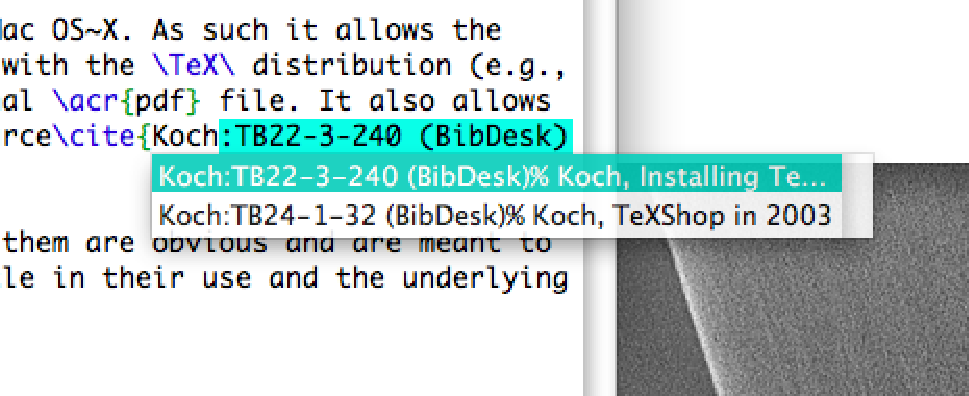
\includegraphics[width=2.7in]{figs/BibDeskPlugin}}\qquad\fbox{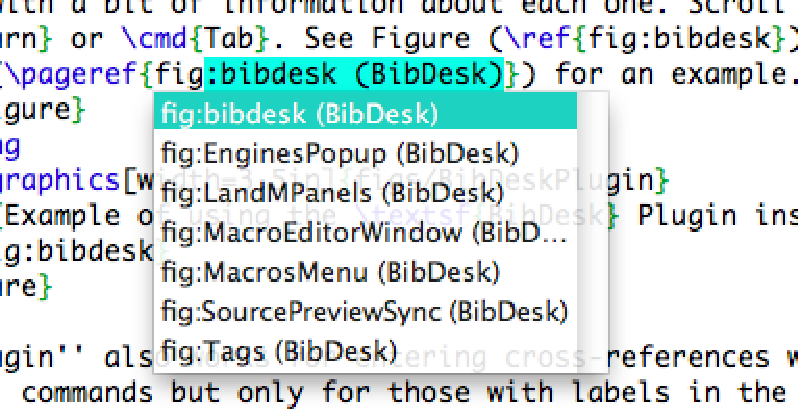
\includegraphics[height=1.2in]{figs/BibDeskPluginXref}}
\caption{Exemples de connexion à \textsf{BibDesk} pour des citations et des références croisées dans \TS.\label{fig:bibdesk}}
\end{figure}
Cette connexion fonctionne également pour la saisie des références croisées dans les commandes \verb|\ref| ou \verb|\pageref|, mais seulement pour celles qui ont des étiquettes dans le fichier que vous éditez.

%The ``plugin'' also works for entering cross-references within \verb|\ref| or \verb|\pageref| commands but only for those with labels in the file you are editing.

\subsection{Aide pour les extensions}
%\subsection{Getting Help for Packages}

Parfois, il peut être utile d'afficher l'aide d'une extension donnée. \TS\ possède une interface avec \texttt{texdoc} qui fera apparaître cette documentation. Cliquez sur \mnu{Aide}\To\mnu{Afficher l'aide pour le package…} (\cmd{Opt-Cmd-I}) et entrez le nom de l'extension.

Vous pouvez, tout aussi aisément, regarder la documentation d'une extension avec la commande \mnu{Aide}\To\mnu{Ouvrir le fichier style…} et entrer le nom complet du fichier \emph{y compris la bonne extension} (p. ex., \texttt{.sty} pour les extensions ou \texttt{.cls} pour les classes de document).

%There are many times when having help about a given package can be handy. \TS\ has an interface to \texttt{texdoc} which will bring up that documentation. Execute the \mnu{Help}\To\mnu{Show Help for Package…} (\cmd{Opt-Cmd-I}) and enter the name of the package.
%
%You can also easily look at a package directly with the \mnu{Help}\To\mnu{Open Style File…} command and enter the full package file name \emph{including the proper extension} (e.g., \texttt{.sty} for packages or \texttt{.cls} for document classes).

% Keyboard Shortcuts
%	For Menu Items via System Preferences->Keyboard & Mouse->Keyboard Shortcuts
%	For built-in frameworks via ~/Library/KeyBindings/DefaultKeyBinding.dict
%	Via editing MainMenu.nib

\section{Maîtrise du clavier}
%\section{Controlling the Keyboard}

Un des meilleurs moyens d'accélérer l'entrée de votre texte dans un fichier source est de garder les mains sur le clavier autant que possible --- c'est une des raisons pour laquelle je n'aime pas l'interface « cliquable » des panneaux LaTeX et Matrix. Il y a beaucoup de raccourcis associés au système de menu de \TS\ mais cette section traite de leurs modifications, de l'ajout d'autres raccourcis, ainsi que d'autres personnalisations du clavier.

%One of the best ways to speed up your entry of text in a source file is to keep your hands on the keyboard as much as possible---only one of the reasons I don't like the ``clicky'' interface of the \LaTeX\ and Matrix Panels. There are many shortcuts associated with the \TS\ menu system but this section is about changing and adding others and other keyboard customizations.

\subsection{Raccourcis de menu et Préférences Système}
%\subsection{Menu Shortcuts \& System Preferences}

Vous souhaiterez, peut-être, créer un raccourci pour un élément de menu qui n'en a pas ou en ajouter un pour une commande dont vous n'aimez pas le raccourci. À partir de Mac~OS~X 10.4 (Tiger) il existe une méthode pour ajouter des raccourcis vers des éléments de menu spécifiques à la fois au niveau global et dans des programmes spécifiques. Cette fonction est devenue beaucoup plus fiable dans OS~X~10.5 et surtout dans OS~X~10.6.

Un exemple en utilisant Mac OS~X~10.6 (Snow Leopard): \TS\ 2.36 a ajouté une commande \mnu{fichier}\To\mnu{Nouveau depuis la papeterie…}, sans un raccourci, qui peut être très utile lorsque vous installez la « papeterie » à votre guise. Pour ajouter \cmd{Opt-Cmd-N} comme raccourci pour cet élément de menu : ouvrez l'application \textsf{Préférences Système…} puis \mnu{Clavier et souris}\To\mnu{Raccourcis clavier} et sélectionnez \mnu{Raccourcis clavier de l'application} ; appuyez sur le bouton \mnu{+} pour ajouter un raccourci ; sélectionnez \TS\ comme application ; entrez le titre exact du menu [\mnu{Nouveau depuis la papeterie…} --- notez que vous \emph{devez} entrer le caractère véritable des points de suspension, «…», (\cmd{Opt-;} avec un clavier anglais, \cmd{Opt-.} avec un clavier français)] ; dès lors, vous pouvez utiliser \cmd{Opt-Cmd-N} comme raccourci.

%Sometimes you'd like to add a shortcut to a menu item that doesn't have one or add one to a command whose shortcut you dislike. Mac~OS~X 10.4 (Tiger) and later have a method to add shortcuts to specific menu items both globally and in specific programs. This feature has become much more reliable in OS~X~10.5 and especially in OS~X~10.6.
%
%One example using Mac~OS~X~10.6 (Snow Leopard): \TS\ 2.36 has added a \mnu{File}\To\mnu{New from Stationery…} command, without a shortcut, which can be very helpful once you set up stationery the way you want. To add \cmd{Opt-Cmd-N} as the shortcut to that menu item: open up the \textsf{System Preferences} application to \mnu{Keyboard}\To\mnu{Keyboard Shortcuts} and select \mnu{Application Shortcuts}; press the \mnu{+} button to add a shortcut; select \TS\ as the application; enter the exact menu title [\mnu{New from Stationery…} --- note you \emph{must} enter a real ellipsis, `…', (\cmd{Opt-;} with the English keyboard layout)]; and press \cmd{Opt-Cmd-N} as the shortcut.

\subsection{Plus d'aide à l'édition}
%\subsection{More Editing Help}

\TS\ est construit en utilisant les interfaces des programmeurs d'Apple (appelées \emph{frameworks}) et hérite donc de toutes les propriétés et de la fonctionnalité de ces interfaces. Il y a beaucoup de choses disponibles dans le \emph{Text framework} qui ne sont pas liées au clavier par défaut ; p. ex., de nombreuses commandes clavier « de type \cmd{emacs} », mais Apple a permis d'ajouter ces commandes à toutes les applications qui utilisent le \emph{Text framework} ; p. ex., \textsf{TextEdit} et \textsf{Mail} ainsi que \TS.

Ceci se fait en créant un fichier spécial, \path{DefaultKeyBinding.dict}, et en le plaçant dans un endroit particulier, \path{~/Library/KeyBindings/} (vous aurez à créer le dossier \path{KeyBindings} à cet endroit s'il n'existe pas déjà).

Vous obtiendrez de plus amples renseignements à ce sujet, ainsi qu'un exemple (utile), en téléchargeant le fichier \path{KeyBindings.zip} depuis <\url{http://public.me.com/herbs2}>.

%\TS\ is built using Apple's programmers interfaces (called frameworks) and therefore inherits all the properties and functionality of those interfaces. There are many things available through the Text framework that aren't tied to the keyboard by default, e.g., many `\cmd{emacs}-like' keyboard commands, but Apple has made it possible to add those commands to all applications that use the Text framework; e.g., \textsf{TextEdit} and \textsf{Mail} as well as \TS.
%
%This is done by creating a special file, \path{DefaultKeyBinding.dict}, and placing it in a particular location, \path{~/Library/KeyBindings/} (you may have to create the \path{KeyBindings} folder there if it doesn't already exist).
%
%You can get more information about this, as well as a (useful) sample, by downloading the \path{KeyBindings.zip} file from <\url{http://public.me.com/herbs2}>.

%\subsection{What is Broken}

% Key Bindings (auto-completion)
%	via ~/Library/TeXShop/Keyboard/autocompletion.plist

\subsection{Raccourcis clavier}
%\subsection{Key Bindings}

Outre l'ajout de raccourcis pour des éléments de menu, vous pouvez, dans \TS{}, réellement lier les frappes de touche afin de les développer dans des groupes de caractères. Pour activer cette fonction, cochez l'option dans  \mnu{TeXShop}\To\mnu{Préférences…}\To\mnu{Document}\To\mnu{Éditeur}\To\ \mnu{Raccourcis clavier}. Vous pouvez également activer ou désactiver cette fonction, pour un document particulier, en utilisant \mnu{Source}\To\mnu{Raccourcis clavier}\To\mnu{Activer/Désactiver}. Cette fonction, auparavant appelée auto-complétion, ne doit pas être confondue avec le complètement de commande --- voir la section~\Vref{sec:CC}, ci-dessous.

%Besides adding shortcuts to Menu Items you can actually bind keystrokes, within \TS, to expand into groups of characters. Checking the \mnu{TeXShop}\To\mnu{Preferences}\To\mnu{Source}\To\mnu{Editor}\To\mnu{Key Bindings} option will enable this feature. You can also toggle it on/off for any particular document using \mnu{Source}\To\mnu{Key Bindings}\To\mnu{Toggle On/Off}. This feature was previously called Auto Completion; not to be confused with Command Completion---see section (\ref{sec:CC}) below.

P. ex., avec un clavier américain, le raccourci \cmd{Opt-,} entre généralement \texttt{\(\leq\)} dans votre document, mais si les raccourcis clavier sont activés, il entrera \verb|\leq|. De même, si vous sélectionnez du texte, en appuyant sur \verb|"| il sera entouré par \verb|``| et \verb|''|.

%E.g., pressing \cmd{Opt-,} with a US keyboard layout, usually enters \texttt{\(\leq\)} into your document but with Key Binding enabled \verb|\leq| will be entered. Similarly, with some text selected pressing \verb|"| will surround the selected text with \verb|``| and \verb|''|.

Vous pouvez ajouter, supprimer ou changer les raccourcis clavier en utilisant l'éditeur (\mnu{Source}\To\mnu{Raccourcis}\To\mnu{Éditer le fichier des raccourcis…}). Les \textsc{Figures}~\ref{fig:keybindingmenu} et \ref{fig:keybindeditor} montrent le menu et l'éditeur de \mnu{Raccourcis}. 
%You can add, remove or change the key bindings using the Key Bindings Editor (\mnu{Source}\To\mnu{Key Bindings}\To\mnu{Edit Key Bindings File…}). Figures (\ref{fig:keybindingmenu}) and (\ref{fig:keybindeditor}) show the \mnu{Key Bindings} Menu and Editor.
\begin{figure}
\centering
\fbox{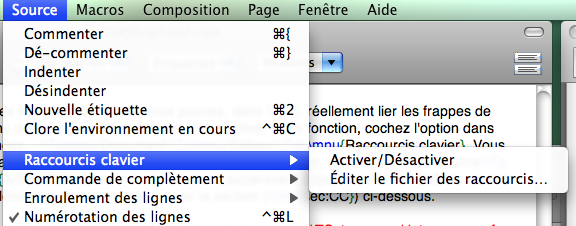
\includegraphics[width=3in]{figs/menuraccourcis}}
\caption{Menu Raccourcis clavier dans \TS.\label{fig:keybindingmenu}}
\end{figure}

\begin{figure}
\centering
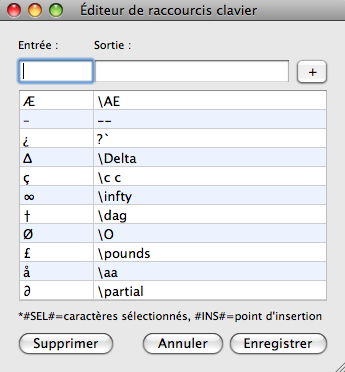
\includegraphics[height=2.00in]{figs/editeurraccourcis}
\caption{Éditeur de raccourcis clavier dans \TS.\label{fig:keybindeditor}}
\end{figure}

%You can add your own keybindings and/or remove those you don't need by editing \path{~/Library/TeXShop/Keyboard/autocompletion.plist}. To add a keybinding to the \verb|_| key so that pressing it with a selection will produce the selection surrounded by \verb|_{| and \verb|}| enter the lines
%\begin{verbatim}
%	<key>_</key>
%	<string>_{#SEL##INS#}</string>
%\end{verbatim}
%to the list in \path{autocompetion.plist}.

% Macros
%	Applescript and Text macros and the Macros Menu

\section{Macros}
%\section{Macros}

Les macros peuvent être de simples substitutions de texte ou des programmes Applescript qui peuvent faire toutes sortes de traitement sur un fichier. Vous pouvez aussi assigner un raccourci clavier à une macro pour une exécution immédiate. Celles qui font partie de \TS\ se trouvent sous le menu \mnu{Macros}.

Vous pouvez supprimer ou ajouter des macros supplémentaires au menu à l'aide du \mnu{Macro Editor} (utilisez la commande \mnu{Macros}\To\mnu{Ouvrir l'éditeur des macros…}). La fenêtre du \mnu{Macro Editor} et les éléments supplémentaires dans le menu \mnu{Macros} sont respectivement présentés dans les \textsc{Figures}~\ref{fig:MacroEditorWindow} et \ref{fig:MacrosMenu}.

Outre l'écriture de vos propres macros, vous pouvez ajouter des macros fournies par des tiers dans le menu \mnu{Macros} de deux façons : soit copier et coller la version texte de la macro dans un \mnu{Nouvel item} du \mnu{Macro Editor}, soit obtenir la macro en tant que fichier \texttt{plist} et l'utiliser avec la commande \mnu{Ajouter une macro à partir du fichier…} trouvée dans le menu \mnu{Macros} lorsque le \mnu{Macro Editor} est ouvert (encore une fois, voir la \textsc{Figure}~\ref{fig:MacrosMenu}).


%Macros can be simple text substitutions or Applescript programs that can do all sorts of processing on a file. You can also assign a keyboard shortcut to any macro for direct execution. The ones that are part of \TS\ are found under the \mnu{Macros} Menu.
%
%You can remove or add additional macros to the menu by using the \mnu{Macro Editor} (use the \mnu{Macros}\To\mnu{Open Macro Editor} command). The \mnu{Macro Editor} window and extra menu items in the \mnu{Macros} Menu are shown in Figures (\ref{fig:MacroEditorWindow}) and (\ref{fig:MacrosMenu}) respectively.
\begin{figure}
\centering
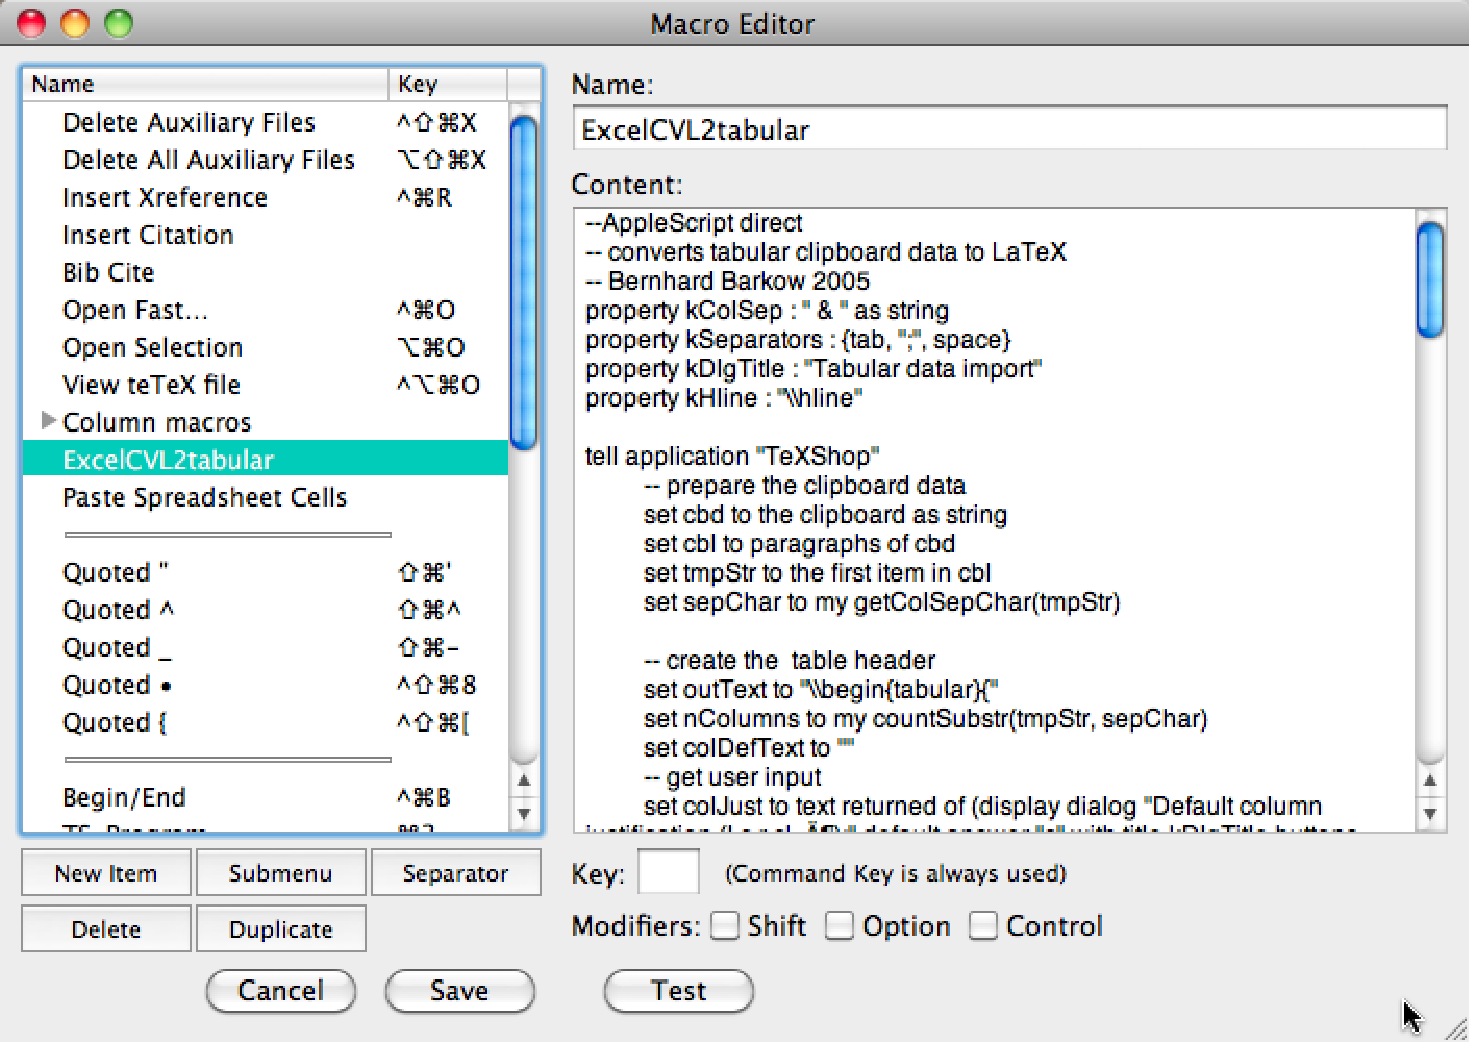
\includegraphics[width=4.75in]{figs/MacroEditorWindow}
\caption{Fenêtre de l'éditeur de macros.}
\label{fig:MacroEditorWindow}
\end{figure}
%
%Besides writing your own macros you can add macros supplied by others to the \mnu{Macros} menu one of two ways: copy and paste the text version of the macro into a \mnu{New Item} in the \mnu{Macro Editor}; or obtain the macro as a \texttt{plist} file and use the \mnu{Add macros from file…} command found in the \mnu{Macros} Menu when the \mnu{Macro Editor} is open (again, see Figure (\ref{fig:MacrosMenu})).

\begin{figure}
\centering
\framebox{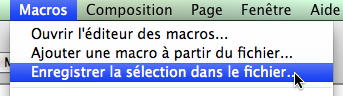
\includegraphics[width=2.25in]{figs/extra}}
\caption{Éléments de menu supplémentaires lorsque l'éditeur de macros est ouvert.\label{fig:MacrosMenu}}
\end{figure}
%\begin{figure}
%\centering
%\framebox{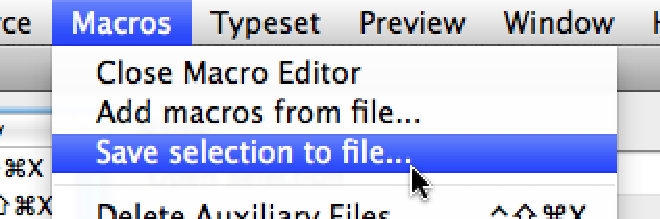
\includegraphics[width=2.5in]{figs/MacrosMenu}}
%\caption{The extra menu items when the Macro Editor is open.}
%\label{fig:MacrosMenu}
%\end{figure}

Pour plus d'informations sur les \cmd{macros} rechercher dans le menu \mnu{Aide}\To\mnu{Aide de TeXShop…}

%More information on macros can be found by searching for \cmd{macros} in \mnu{Help}\To\mnu{TeXShop Help Panel…}.

\subsection{Macros de texte}
%\subsection{Text Macros}

Les macros de texte sont de simples substitutions de texte. Vous pouvez aussi dire à \TS\ d'insérer n'importe quel texte sélectionné en utilisant \verb|##SEL|, de placer le curseur à l'aide \verb|##INS| et même de mettre la macro elle même sur plusieurs lignes. Ensuite, vous pouvez affecter la macro de texte à un raccourci clavier.

J'aime utiliser \cmd{Cmd-B} et \cmd{Cmd-I} pour insérer \verb|\textbf{…}| et \verb|\emph{…}| dans le document où \texttt {...} est n'importe quel texte sélectionné. Les macros pour faire cela sont déjà dans le menu \mnu{Macros}\To\mnu{Text Styles} ; donc, il ne nous reste plus qu'à leur attribuer des raccourcis clavier. Pour attribuer \cmd{Cmd-I} à la macro \mnu{emphasize} : ouvrir le \mnu{Macro Editor} où la forme du menu \mnu{Macros} apparaît dans le volet de gauche, cliquez sur la macro \mnu{emphasize} qui se trouve sous \mnu{Text Styles} ; cliquez sur la case d'insertion de la clé (\mnu{Touche}) où il suffit d'insérer un « \texttt{i} » minuscule (la touche \cmd{cmd} est toujours prise en charge et des touches de modification supplémentaires peuvent être cochées).

%Text macros are simple text substitutions. You can also tell \TS\ to insert any selected text using \verb|#SEL#|, place the cursor using \verb|#INS#| and even put in multiple lines in the macro itself. Then you can assign the text macro to a keyboard shortcut.
%
%I like to use \cmd{Cmd-B} and \cmd{Cmd-I} to insert \verb|\textbf{…}| and \verb|\emph{…}| into the document where \texttt{…} is any possible selected text. Macros to do that are already under the \mnu{Macros}\To\mnu{Text Styles} Menu so we need only assign keyboard shortcuts to them. To assign \cmd{Cmd-I} to the \mnu{emphasize} macro: open the \mnu{Macro Editor} where the form of the \mnu{Macros} menu appears in the left hand pane; click the \mnu{emphasize} macro found under \mnu{Text Styles}; click the Key insertion box and simply insert a lower case `\texttt{i}' (the \cmd{Cmd} key is assumed and additional modifier keys can be checked off).

\subsection{Macros Applescript}
%\subsection{Applescript Macros}

Dans le menu \mnu{Macros}, il n'est pas possible de distinguer les macros Applescript des macros de texte, pourtant elles peuvent faire des traitements compliqués et ajouter ou modifier le fichier source dans \TS{}. P. ex., la macro \mnu{Program}, définie par défaut, crée la ligne suivante
\begin{verbatim}
%! TEX TS-program = xxxx
\end{verbatim}
en tête d'un fichier avec le moteur de votre choix à la place de \texttt{xxxx}. Vous pouvez voir le code Applescript de cette macro en cliquant sur son nom dans l'éditeur de macros (\mnu{Macro Editor}). 

%You cannot distinguish Applescript macros in the \mnu{Macros} Menu from text macros but they can do complicated processing and add/change the source file in \TS. One example in the default set is the \mnu{Program} macro that creates a
%\begin{verbatim}
%% !TEX TS-program = xxxx
%\end{verbatim}
%line at the top of a file with your choice of engine substituted for \texttt{xxxx}. You can look at the Applescript code for this macro by clicking on its name in the \mnu{Macro Editor}.

%\begin{figure}[h]
%\centering
%\framebox{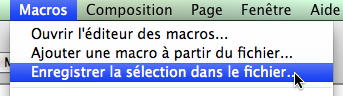
\includegraphics[width=2.25in]{figs/extra}}
%\caption{Éléments de menu supplémentaires lorsque l'éditeur de macros est ouvert.\label{fig:MacrosMenu}}
%\end{figure}

% Command Completion
%	via ~/Library/TeXShop/CommandCompletion.txt & Macros

\section{Complètement de commande}\label{sec:CC}
%\section{Command Completion}\label{sec:CC}

Le balisage de \LaTeX\ est plutôt prolixe ce qui est agréable, car il décrit ce qu'il est censé faire, mais un peu pénible à écrire. Le complètement de commande vous permet d'insérer des environnements complets et des commandes en quelques frappes suivies d'une ou plusieurs pressions  sur la touche de déclenchement (qui est, par défaut, \cmd{Esc} mais peut être remplacée par \cmd{Tab} en allant dans \mnu{TeXShop}\To\mnu{Préférences…}\To\mnu{Document}\To\mnu{Commande de complétion déclenchée par}).

Les commandes avec arguments ont généralement un repère (\texttt{•}) placé à leur niveau. Pour aller à l'argument suivant, utilisez la commande \mnu{Source}\To\ \mnu{Commande de complètement}\To\mnu{Repères} \To\mnu{Repère suivant} (\cmd{Ctl-Cmd-F} [ou \cmd{Opt-Esc/Tab}]). Ceci sélectionne en même temps le repère pour qu'il soit automatiquement remplacé par l'information saisie. Voir la documentation complète, avec les listes de commandes et abréviations, fournie avec \TS\ dans le dossier \path{~/Library/TeXShop/CommandCompletion/}, pour plus d'informations.

%\LaTeX\ markup is rather wordy which is nice because it describes what it's supposed to do but a bit painful to write. Command Completion allows you to insert complete environments and commands with a few keystrokes and the press of a ``trigger'' key (this is \cmd{Esc} by default but can be changed to \cmd{Tab} in \mnu{TeXShop}\To\mnu{Preferences}\To\mnu{Source}\To\mnu{Command Completion Triggered By:}).

%Commands that have arguments usually have a Mark (\texttt{•}) inserted for each argument. You move to the next argument by using the \mnu{Source}\To\mnu{Command Completion}\To\mnu{Marks}\To\mnu{Next Mark} command (\cmd{Ctl-Cmd-F} [or \cmd{Opt-Trigger}]). This also selects the Mark so typing automatically removes the Mark and substitutes the typed information. See the complete documentation, with lists of commands/abbreviations supplied with \TS\ out of the box, in the \path{~/Library/TeXShop/CommandCompletion/} folder for much more information.

\subsection{Complètement}
%\subsection{Completions}

Vous pouvez compléter de nombreuses commandes en commençant à les saisir puis en appuyant sur la touche de déclenchement. Les commandes qui diffèrent par leur nombre d'arguments optionnels sont générées par des pressions successives sur la touche de déclenchement. Ainsi, taper \verb|\sec| puis la touche de déclenchement, sur une nouvelle ligne, produit

%You can complete many commands by starting to type them and pressing the trigger key. Variations on the commands with differing numbers of optional arguments are generated by additional presses of the trigger. One example: typing \verb|\sec| and then the trigger on a new line produces
\begin{verbatim}
\section{|selmark}
\end{verbatim}
tandis qu'une seconde pression sur la touche de déclenchement donne
%while a second press of the trigger gives
\begin{verbatim}
\section*{|selmark}
\end{verbatim}
la variante étoilée (*) et qu'une dernière pression de cette touche donne la commande
%the *-variant of the command and a final press of the trigger gives
\begin{verbatim}
\section[|selmark]{•}
\end{verbatim}
avec l'argument optionnel.
%with the optional argument.

\subsection{Substitutions ou abréviations}
%\subsection{Substitutions or Abbreviations}

Outre le complètement des commandes entrées partiellement, il y a aussi de nombreuses abréviations. Celles-ci sont de courts mnémoniques pour accéder à des substitutions complètes.

Toutes les abréviations pour les environnements commencent par un « \texttt{b} ». Pour obtenir l'environnement  \cmd{itemize} complet, entrez \verb|\bite| sur une nouvelle ligne et appuyez sur la touche de déclenchement ce qui produira

%Besides completions for partial command insertions there are also many abbreviations. These are short mnemonics for complete substitutions. 
%
%All abbreviations for environments start with a `\texttt{b}'. To generate a complete \cmd{itemize} environment place \verb|\bite| on a line by itself and press the trigger key to get
\begin{verbatim}
\begin{itemize}
\item
|selmark
\end{itemize}•
\end{verbatim}
terminé par un repère pour que vous puissiez facilement accéder à la fin de l'environnement. Des items supplémentaires peuvent être créés en tapant \verb|\it| puis la touche de déclenchement afin d'obtenir
%with an extra Mark at the end so you can easily jump to the end of the environment. Additional items can be generated by typing \verb|\it| and the trigger to get
\begin{verbatim}
\item
|selmark
\end{verbatim}
prêt pour l'entrée d'un texte.
%ready for entry of text.

En outre, les commandes de sous-sectionnement possèdent leurs abréviations. Elles peuvent être obtenues en tapant  \verb|\ssec| puis en pressant la touche de déclenchement ce qui donnera

%In addition to the \verb|\section| command lower level sectioning commands have abbreviations. Sub-sections can be generated by typing \verb|\ssec| and the trigger to get
\begin{verbatim}
\subsection{|selmark}
\end{verbatim}
des pressions successives sur la touche de déclenchement donneront, la variante étoilée (*) et, enfin, la variante avec l'argument optionnel.
%with subsequent presses of the trigger key giving the *-variant and finally the variant with the optional argument.

En dernier exemple, l'entrée de \verb|\tt| suivi d'une pression sur la touche de déclenchement donnera la commande \verb|\texttt{|\selmark\verb|}| ; une seconde pression de cette la touche donnera la déclaration \verb|\ttfamily| : des résultats similaires sont obtenus avec les autres commandes de changement de style de police.

%As a final example \verb|\tt| and the trigger gives the \verb|\texttt{|\selmark\verb|}| command and a second press of the trigger gives the declaration \verb|\ttfamily| with similar results for other font changing commands.

\subsection{Hé !, ça ne marche pas !}
%\subsection{Hey, it doesn't work!}

Si ces exemples ne fonctionnent pas, vous devrez probablement permettre à \TS\ de mettre à jour le dossier \path{~/Library/TeXShop/CommandCompletion/} ; supprimez purement et simplement ce dossier de \path{~/Library/TeXShop/} et redémarrez \TS.

%If these examples don't work you probably need to let \TS\ update the \path{~/Library/TeXShop/CommandCompletion/} folder; simply delete that folder from \path{~/Library/TeXShop/} and restart \TS.

% Engines
%	via ~/Library/TeXShop/Engines/

\section{Extension du traitement par les moteurs}
%\section{Extending Processing via Engines}

\TS\ propose plusieurs « moteurs » par défaut (aussi appelée « scripts », ce qui n'a pas changé depuis l'origine) dans son menu \mnu{Composition}. Ils comprennent, notamment, \mnu{Plain TeX} ou \mnu{LaTeX} (soit en utilisant \texttt{pdftex} ou \texttt{TeX+DVI}), \mnu{BibTeX}, \mnu{MakeIndex}, \mnu{MetaPost} ou \mnu{ConTeXt}. Mais, dans ce que vous souhaiterez faire, beaucoup de choses ne relèveront pas de cette offre limitée ; si bien que \TS\ vous permet également d'installer de nouveaux moteurs qui sont stockés dans \path{~/Library/TeXShop/Engines/}. Ces moteurs supplémentaires n'apparaissent pas dans le menu \mnu{Composition}, mais seulement dans la liste déroulante de la barre d'outils du source (voir la \textsc{Figure}~\ref{fig:EnginesPopup}).

Vous pouvez utiliser ces moteurs en les sélectionnant dans cette liste déroulante, puis en appuyant sur le bouton \mnu{Composition} ou mieux, si vous utilisez différents moteurs pour différents documents, en mettant une ligne comme

%\TS\ offers several default ``engines'' (also referred to as ``scripts'' which is left over from earlier times) in its \mnu{Typeset} Menu. These include running \mnu{Plain TeX} or \mnu{LaTeX} (either using \texttt{pdftex} or \texttt{TeX+DVI}), \mnu{BibTeX}, \mnu{MakeIndex}, \mnu{MetaPost} or \mnu{ConTeXt}. But there are many things you may wish to do that fall outside of this limited set so \TS\ also allows you to create new engines that are stored in \path{~/Library/TeXShop/Engines/}. These additional engines do not show up in the \mnu{Typeset} menu but only in the popup list on the Source and Preview Toolbar (see Figure (\ref{fig:EnginesPopup})). 
%
%You can use these engines by choosing from that popup list and then pressing the Typeset button or, a better choice if you use different engines for different documents, by putting a line like
\begin{verbatim}
% !TEX TS-program = xelatex
\end{verbatim}
en tête de votre fichier source ; dans cet exemple le moteur \texttt{xelatex} sera utilisé pour ce fichier indépendamment des autres choix.
%at the top of your source file; the example given will run the \texttt{xelatex} engine on this file independent of other choices.

D'origine, seuls quelques moteurs sont activés dans \TS\ (c.-à-d., directement dans le dossier \path{~/Library/TeXShop/Engines/}), mais il y a aussi d'autres moteurs dans le dossier \path{~/Library/TeXShop/Engines/Inactive/}. À titre d'exemple, nous allons activer et utiliser le moteur \cmd{pdflatexmk} trouvé dans \path{~/Library/TeXShop/Engines/Inactive/Latexmk/}.

%\TS\ is shipped with a few engines activated (i.e., directly in the \path{~/Library/TeXShop/Engines/} folder) but also includes several additional ones in \path{~/Library/TeXShop/Engines/Inactive/}. As an example let's activate and use the \cmd{pdflatexmk} engine found in \path{~/Library/TeXShop/Engines/Inactive/Latexmk/}.
\begin{figure}
\centering
\framebox{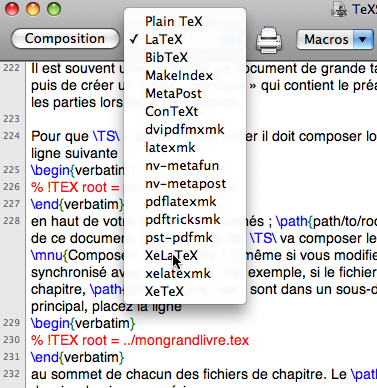
\includegraphics[width=2.0in]{figs/moteurs}}
\caption{Menu déroulant des moteurs dans la barre d'outils du source.\label{fig:EnginesPopup}}
\end{figure}

\subsection{Moteur \texttt{pdflatexmk}}
%\subsection{The \texttt{pdflatexmk} engine}

Si votre document comportait des références croisées, des bibliographies ou des index, il faudrait plusieurs compilations avec \texttt{pdflatex}, mais aussi d'autres encore avec \texttt{bibtex} ou \texttt{makeindex}, pour créer les bibliographies, les index et résoudre toutes les références croisées. Le moteur \texttt{pdflatexmk} automatise ce processus.

Pour activer ce moteur il suffit de déplacer le fichier \texttt{pdflatexmk.engine} du répertoire \path{~/Library/TeXShop/Engines/Inactive/Latexmk/} pour le mettre, deux dossiers en amont, dans \path{~/Library/TeXShop/Engines/}. Au redémarrage de \TS\ vous pourrez vérifier que \cmd{pdflatexmk} figure maintenant dans le menu déroulant.

%If your document had cross-references, bibliographies or indexes it takes multiple \texttt{pdflatex} runs with intermediate runs of \texttt{bibtex} and/or \texttt{makeindex} to create the bibliographies, indexes and resolve all cross-references. The \texttt{pdflatexmk} engine automates this whole process.
%
%To activate the engine simply move the \texttt{pdflatexmk.engine} file from \path{~/Library/TeXShop/Engines/Inactive/Latexmk/} two folders up, to \path{~/Library/TeXShop/Engines/}. When you restart \TS\ you can check that \cmd{pdflatexmk} in now in the popup menu.

%Now place the line
Il ne reste plus qu'à entrer la ligne
\begin{verbatim}
% !TEX TS-program = pdflatexmk
\end{verbatim}
en tête de votre fichier source. Dès cet instant, il suffit de composer le fichier (\mnu{Composition}\To{} \mnu{Composer} or \cmd{Cmd-T}) pour que \TS\ utilise ce moteur et que le processus complet de mise en page du document s'effectue jusqu'à sa forme finale. 
%at the top of your source file. From then on when you simply typeset the file (\mnu{Typeset}\To\mnu{Typeset} or \cmd{Cmd-T}) \TS\ will use this engine and the complete process for typesetting the document to its final form will be carried out.

\end{document}
